\documentclass[tikz]{standalone}

\usepackage{tikz}
\usepackage{ifthen}
\pgfdeclarelayer{back}
\pgfsetlayers{back,main}
\usetikzlibrary{math} %needed tikz library

%
% Customize colors
%
\definecolor{chapter-color}{cmyk}{1, 0.50, 0, 0.25}
\definecolor{link-color}{cmyk}{1, 0.50, 0, 0.25}
\definecolor{cite-color}{cmyk}{0, 0.7, 0.9, 0.2}
\definecolor{codegreen}{rgb}{0,0.6,0}
\definecolor{codegray}{rgb}{0.5,0.5,0.5}
\definecolor{codepurple}{rgb}{0.58,0,0.82}
\definecolor{backcolour}{rgb}{0.95,0.95,0.92}
\definecolor{codebgcolor}{RGB}{129, 139, 152}
\definecolor{codehighlightcolor}{RGB}{255, 230, 153}
%\definecolor{codegreen}{RGB}{0, 153, 0}
%\definecolor{codegray}{RGB}{127, 127, 127}
\definecolor{codeblue}{RGB}{102, 214, 237}
\definecolor{codekeyword}{RGB}{249, 36, 114}
\definecolor{codecomment}{RGB}{127, 127, 127}
\definecolor{backcolor}{RGB}{242, 242, 235}
\definecolor{linkcolor}{RGB}{102, 0, 0}
\definecolor{corange}{RGB}{255, 70, 0}
\definecolor{cyellow}{RGB}{209, 153, 0}
\definecolor{cblue}{RGB}{64, 128, 255}
\definecolor{cbrown}{RGB}{153, 102, 51}
\definecolor{cpink}{RGB}{255, 0, 255}
\definecolor{cred}{RGB}{255, 64, 0}
\definecolor{cgreen}{RGB}{0, 191, 0}
\definecolor{clightblue}{RGB}{191, 217, 255}
\definecolor{cturquois}{RGB}{0, 255, 255}
\definecolor{cpurple}{RGB}{128, 0, 255}
\definecolor{clightgreen}{RGB}{175, 255, 175}
\definecolor{clightgray}{RGB}{211, 211, 211}
\definecolor{clightpink}{RGB}{255, 175, 255}
\definecolor{cdarkblue}{RGB}{0, 0, 255}
\definecolor{cdarkred}{RGB}{255, 0, 0}
\definecolor{cdarkgreen}{RGB}{0, 255, 0}
\definecolor{cgray}{RGB}{153, 153, 153}

\definecolor{myblue}{RGB}{55, 126, 184}
\definecolor{myorange}{RGB}{255, 127, 0}
\definecolor{myred}{RGB}{228, 26, 28}
\definecolor{mypurple}{RGB}{152, 78, 163}
\definecolor{mygreen}{RGB}{77, 175, 74}
\definecolor{myyellow}{RGB}{255, 255, 51}
\definecolor{mybrown}{RGB}{166, 86, 40}
\definecolor{mypink}{RGB}{166, 86, 40}
\definecolor{mygray}{RGB}{153, 153, 153}


\makeatletter
\pgfkeys{%
  /tikz/on layer/.code={
    \def\tikz@path@do@at@end{\endpgfonlayer\endgroup\tikz@path@do@at@end}%
    \pgfonlayer{#1}\begingroup%
  }%
}
\makeatother

\begin{document}

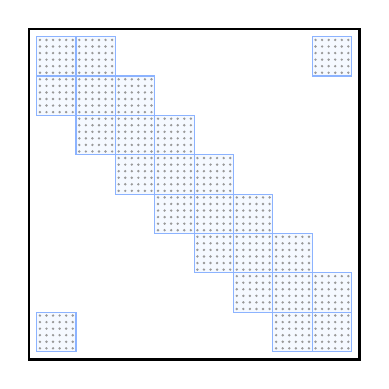
\begin{tikzpicture}

\tikzmath{
\volume = 8; % volume of the 1D lattice
\slimit = \volume -1;
\size = 4.0; % size in points
\step = \size / \volume;
\ndots = 6; % dots per square
\dlimit = \ndots -1;
\dstep = \step / \ndots;
} 

\draw[black, thick] (-0.1,-0.1) rectangle (\size+0.1,\size+0.1);

% for orientation
%\filldraw[red] (0.0,0.0) circle (1.0pt);
%\filldraw[green] (1.0,0.0) circle (1.0pt);
%\filldraw[yellow] (0.0,1.0) circle (1.0pt);

\foreach \c in {0,...,\slimit} {
    \coordinate (A1) at (\c*\step+0.0,  \size-\step-\c*\step);
    \coordinate (B1) at (\c*\step+\step,\size-\c*\step);

    \ifthenelse{\c=\slimit}{
        \coordinate (A2) at (0.0,       \size-\step-\c*\step);
        \coordinate (B2) at (\step,       \size-\c*\step);
        \coordinate (A3) at (\c*\step+0.0,\size-\step);
        \coordinate (B3) at (\c*\step+\step,\size);
    }{
        \coordinate (A2) at (\c*\step+1*\step,\size-\step-\c*\step);
        \coordinate (B2) at (\c*\step+2*\step,\size-\c*\step);
        \coordinate (A3) at (\c*\step+0*\step,\size-2*\step-\c*\step);
        \coordinate (B3) at (\c*\step+1*\step,\size-\step-\c*\step);
    }
    
    \draw[color=cblue!60, fill=cblue!5, thin, on layer=back] (A1) rectangle (B1);
    \draw[color=cblue!60, fill=cblue!5, thin, on layer=back] (A2) rectangle (B2);
    \draw[color=cblue!60, fill=cblue!5, thin, on layer=back] (A3) rectangle (B3);

    \foreach \x in {0,...,\dlimit} {
        \foreach \y in {0,...,\dlimit} {
            % diagonal dots
            \coordinate (C) at (\x*\dstep+0.5*\dstep+\c*\step,\y*\dstep+\size-\step+0.5*\dstep-\c*\step);

            \ifthenelse{\c=0}{
                \coordinate (O1) at (\x*\dstep+\size-\step+0.5*\dstep+\c*\step,\y*\dstep+\size-\step+0.5*\dstep-\c*\step);
            }{
                \coordinate (O1) at (\x*\dstep-\step+0.5*\dstep+\c*\step,\y*\dstep+\size-\step+0.5*\dstep-\c*\step);
            }

            \ifthenelse{\c=\slimit}{
                \coordinate (O2) at (\x*\dstep+0.5*\dstep,\y*\dstep+\size-\step+0.5*\dstep-\c*\step);
            }{
                \coordinate (O2) at (\x*\dstep+\step+0.5*\dstep+\c*\step,\y*\dstep+\size-\step+0.5*\dstep-\c*\step);
            }

            \filldraw[cgray] (C) circle (0.2pt);
            \filldraw[cgray] (O1) circle (0.2pt);
            \filldraw[cgray] (O2) circle (0.2pt);

        };
    };
};

\end{tikzpicture}

\end{document}